% 建议使用 XeLaTeX 或 LuaLaTeX 编译(更佳的中文支持)
\documentclass[UTF8,zihao=-4]{ctexart}

% 统一导言
\usepackage[a4paper,margin=2.5cm]{geometry}
\usepackage{amsmath,amssymb,amsthm}
\usepackage{bm}
\usepackage{hyperref}
\usepackage{graphicx}
\usepackage{caption}
\usepackage{listings}
\usepackage{xcolor}
\usepackage{float}
\usepackage{placeins}

% 图片路径
\graphicspath{{figures/}}

% 统一代码风格
\lstdefinestyle{code}{%
  language=Python,
  basicstyle=\ttfamily\small,
  numbers=left,
  numberstyle=\tiny,
  keywordstyle=\color{blue}\bfseries,
  commentstyle=\color{teal!70!black},
  stringstyle=\color{orange!70!black},
  breaklines=true,
  frame=single,
  rulecolor=\color{black!30},
  tabsize=2,
  showstringspaces=false
}
\lstset{style=code}

\title{随机森林:理论与实践}
\author{}
\date{\today}

\begin{document}
\maketitle

% 结构:Introduction / Theory and Formulas / Applications and Tips / Python Practice / Result / Summary

\section{引言}
随机森林(Random Forest)是基于“装袋”(bagging)与“特征子采样”的集成学习方法。它通过对多个随机化的决策树进行投票(分类)或求均值(回归),显著降低方差、提升泛化能力,同时对数据预处理的要求较低。

\section{原理与公式}
随机森林的两大关键:\emph{自助采样}(bootstrap)与\emph{特征子采样}(每次划分仅在随机抽取的特征子集上搜索最优划分)。设有 $B$ 棵树 $\{T_b\}_{b=1}^B$,每棵树在各自的自助样本 $\mathcal{D}_b$ 上训练。
分类任务的集成预测为多数表决:
\begin{equation}
\hat{y} = \mathrm{mode}\big( T_1(\mathbf{x}),\dots,T_B(\mathbf{x}) \big),
\end{equation}
回归任务的集成预测为简单平均:
\begin{equation}
\hat{y} = \frac{1}{B} \sum_{b=1}^B T_b(\mathbf{x}).
\end{equation}
由于特征子采样降低了各基学习器的相关性,随着树数 $B$ 的增加,整体方差可进一步下降。分类中常用的经验选择是 \texttt{max\_features}=$\sqrt{p}$($p$ 为特征数)。

\textbf{袋外(OOB)估计:} 每次自助采样平均会留下约 $\approx 36\%$ 的“袋外”样本。利用袋外样本做内部验证可得到接近无偏的泛化评估,无需额外划分验证集或交叉验证。

常用超参数包括:树的数量 $B$(\texttt{n\_estimators})、每次划分考虑的特征数(\texttt{max\_features})、树深与叶子最小样本数(正则化)、以及 \texttt{bootstrap}/\texttt{oob\_score} 设置等。

\section{应用与技巧}
\begin{itemize}
  \item \textbf{优点:} 默认表现强、鲁棒性好、对特征尺度不敏感、能处理混合类型特征。
  \item \textbf{缺点:} 预测与存储开销较单棵树更大;可解释性低于浅层树。
  \item \textbf{正则化与调参:} 调整 \texttt{max\_depth}、\texttt{min\_samples\_leaf}、\texttt{max\_features};增大 \texttt{n\_estimators} 直至 OOB/测试指标收敛。
  \item \textbf{诊断:} 使用 OOB 分数、随树数变化的学习曲线;查看特征重要性(必要时用置换重要性)。
  \item \textbf{预处理:} 类别特征需独热编码;数值特征一般无需标准化。
\end{itemize}

\section{Python 实战}
在本章节目录运行下述命令,图片将保存到 \texttt{figures/}:
\begin{lstlisting}[style=code,caption={生成随机森林配图},label={lst:genfigs_rf_cn}]
python gen_random_forest_figures.py
\end{lstlisting}

% 纳入完整 Python 源码
\lstinputlisting[style=code,caption={gen\_random\_forest\_figures.py 源码},label={lst:source_rf_cn}]{gen_random_forest_figures.py}

\section{结果}
\begin{figure}[H]
  \centering
  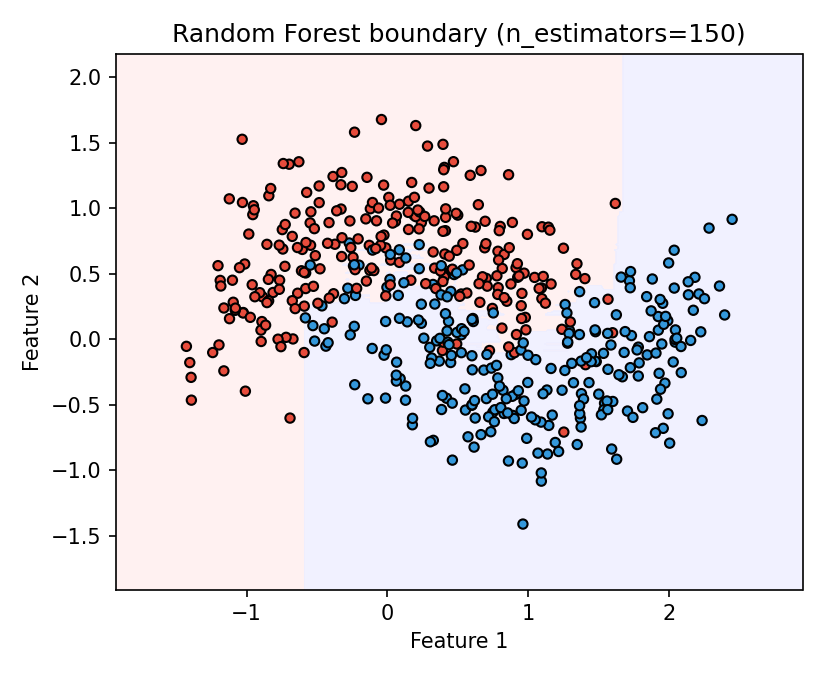
\includegraphics[width=0.9\linewidth]{rf_decision_boundary_2class.png}
  \caption{随机森林在两类数据上的决策边界。}
  \label{fig:rf2_cn}
\end{figure}
\FloatBarrier

\begin{figure}[H]
  \centering
  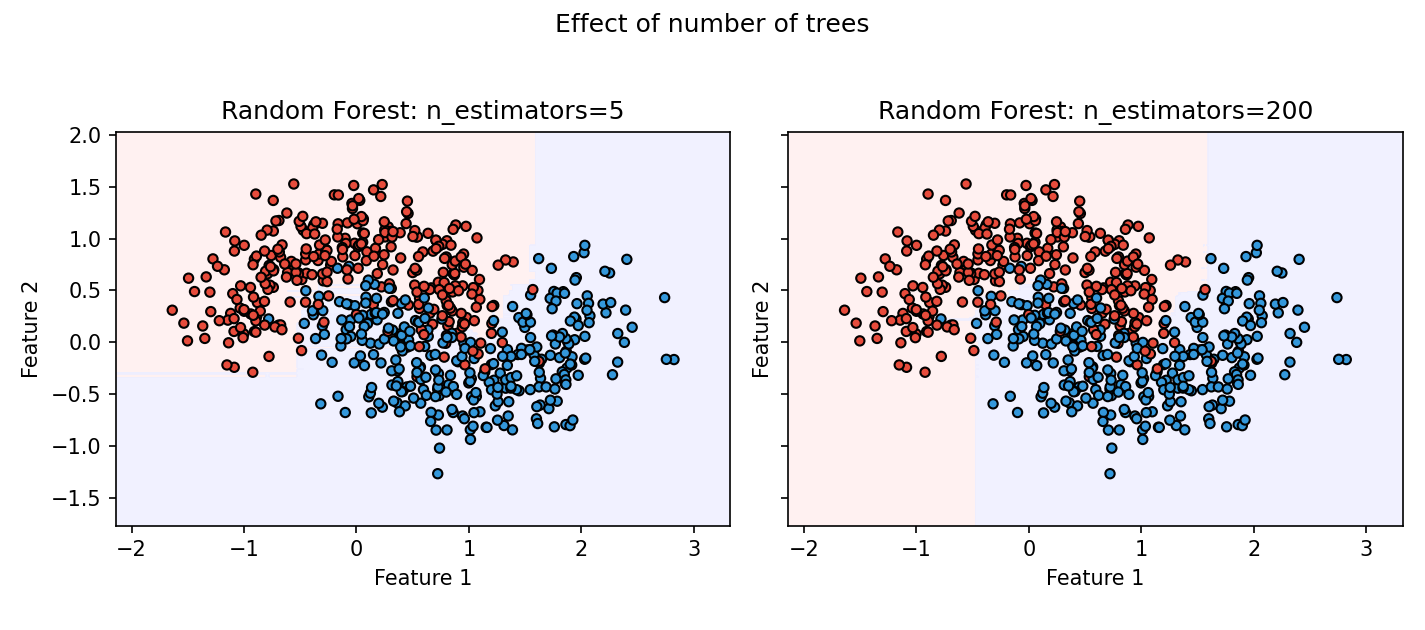
\includegraphics[width=0.95\linewidth]{rf_n_estimators_compare.png}
  \caption{树数量影响:少树 vs 多树的对比。}
  \label{fig:rf_n_cn}
\end{figure}
\FloatBarrier

\begin{figure}[H]
  \centering
  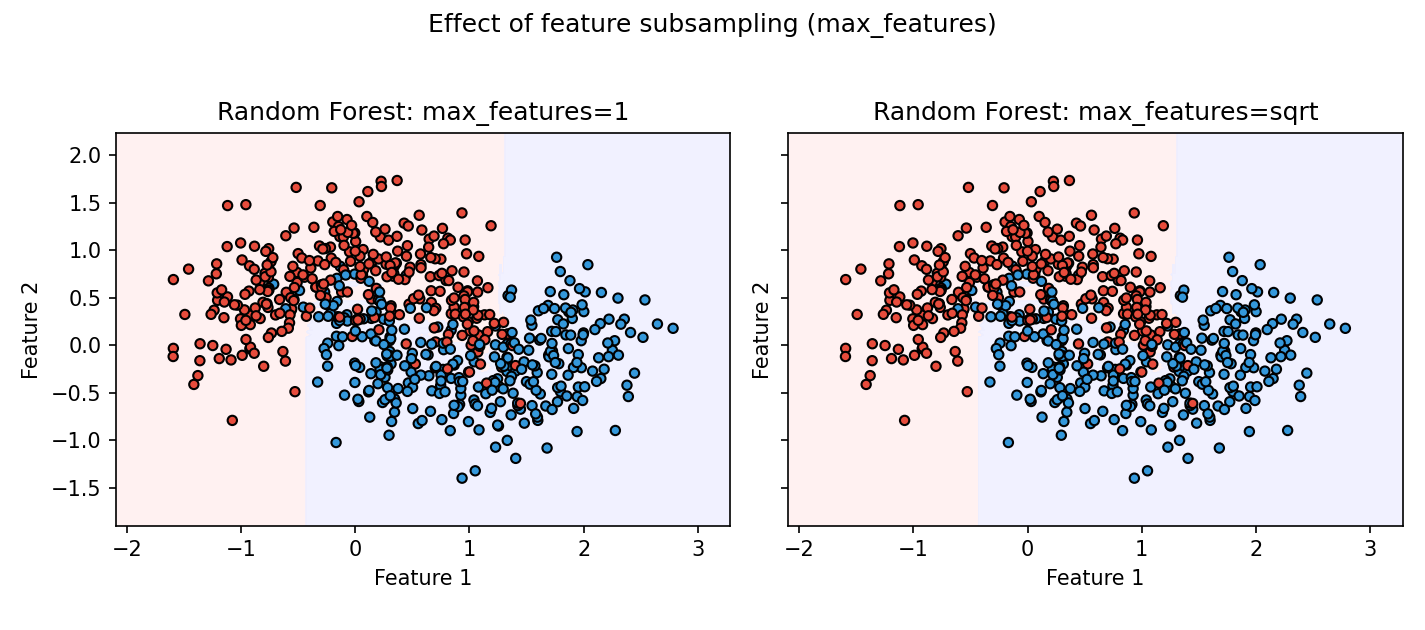
\includegraphics[width=0.95\linewidth]{rf_max_features_compare.png}
  \caption{不同 \texttt{max\_features} 下的决策边界对比。}
  \label{fig:rf_mf_cn}
\end{figure}
\FloatBarrier

\begin{figure}[H]
  \centering
  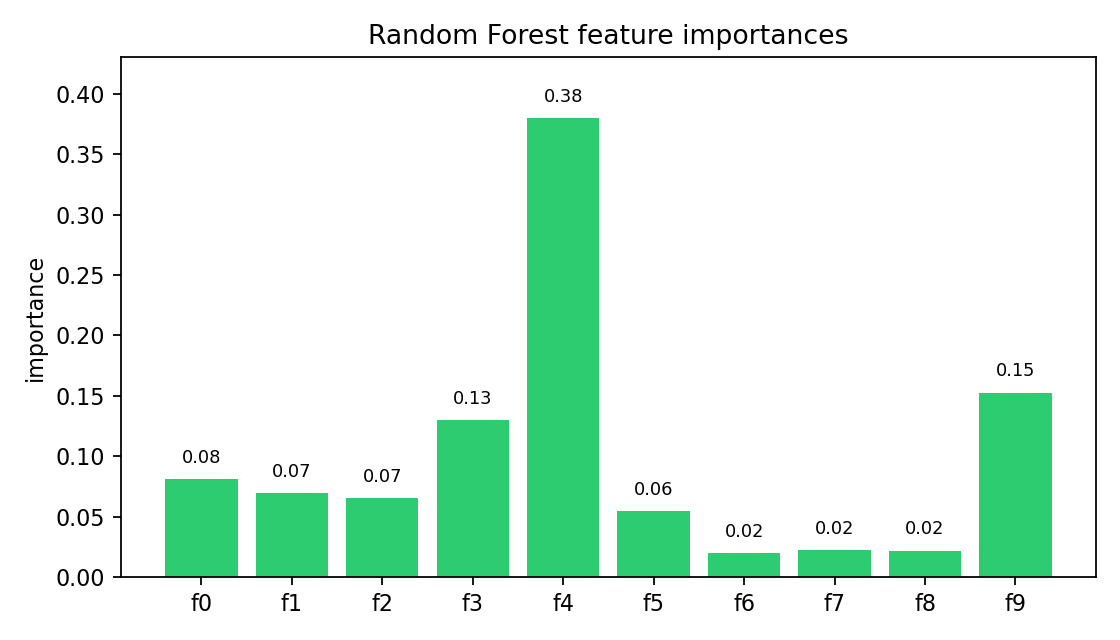
\includegraphics[width=0.85\linewidth]{rf_feature_importances.png}
  \caption{随机森林的特征重要性可视化。}
  \label{fig:rf_fi_cn}
\end{figure}
\FloatBarrier

\begin{figure}[H]
  \centering
  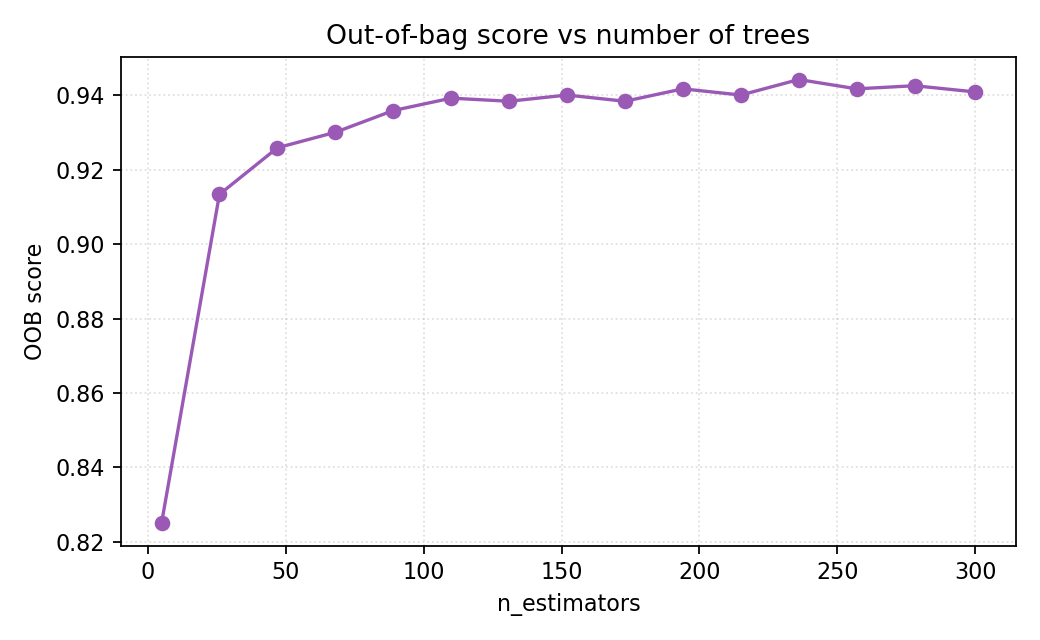
\includegraphics[width=0.85\linewidth]{rf_oob_curve.png}
  \caption{袋外(OOB)分数随树数量变化的曲线。}
  \label{fig:rf_oob_cn}
\end{figure}
\FloatBarrier

\section{总结}
随机森林通过“装袋 + 特征子采样”有效降低方差,提供 OOB 内部验证与可用的特征重要性,是工程中可靠的通用基线模型。通过合适的树数与正则化参数,可在准确率与效率之间取得良好平衡。

\end{document}

